\documentclass[aspectratio=169]{beamer}

\usepackage[T1]{fontenc}
\usepackage[utf8]{inputenc}
\usepackage[american]{babel}
\usepackage{amsmath,amsthm}
\usepackage{unicode}
\usepackage{tikz}
\usetikzlibrary{calc}%matrix,decorations,decorations.text,calc,arrows,snakes,shapes,positioning}
\usepackage{multimedia}

\mode<presentation>{%
  \usetheme{ibm}
}


\title{SIDH Proof of Knowledge}
\author[De Feo, Dobson, Galbraith, Zobernig]{\underline{Luca De Feo}\footnotemark[1], Samuel Dobson\footnotemark[2], Steven D. Galbraith\footnotemark[2], Lukas Zobernig\footnotemark[2]}
\institute[]{\footnotemark[1]IBM Research Europe, Switzerland\\
  \footnotemark[2]Mathematics Department, University of Auckland, New Zealand}
\date[Dec 6, 2022, Asiacrypt]{December 6, 2022, Asiacrypt, Taipei}

\begin{document}

\frame[plain]{\titlepage}

%%

\begin{frame}{Proofs of Isogeny Knowledge\dots Why?}
  \large
  {\Large
    \[\phi : E_0 \longrightarrow E_1\]}
  \begin{itemize}
    \setlength{\itemsep}{1em}
  \item Signatures,
  \item Verifiable \textcolor{gray}{\sl<insert your favorite primitive>},
  \item Non-interactive SIDH (\raisebox{-.4ex}{\LARGE\textdagger{}}) key exchange,
  \item \dots Why not?
  \end{itemize}
\end{frame}

%%

\begin{frame}
  \large
  \centering
  \begin{tikzpicture}
    \node (E0) at (0,0) {\Large$E_0$};
    \node (E1) at (6,0) {\Large$E_1$};
    \node at (3,1) {\Large$\phi$};
    
    \begin{uncoverenv}<-2>
      \draw[dashed,-latex] (E0) edge (E1);
    \end{uncoverenv}
    \begin{uncoverenv}<2->
      \color{gray}
      \node (c0) at (-2,2) {\parbox{9em}{supersingular curve\\ $y^2 = x^3 -6x^2 + x$}};
      \node (c1) at (8,2) {\parbox{9em}{supersingular curve\\ $y^2 = x^3 + 371x^2 + x$}};
      \draw[->]
      (c0) edge[bend right=50] (E0)
      (c1) edge[bend left=50] (E1);      
    \end{uncoverenv}
    \begin{uncoverenv}<3->
      \foreach \i in {1,...,4} {
        \pgfmathparse{(-1)^\i}
        \node (w\i) at (1.2*\i,0.3*\pgfmathresult) {$\bullet$};
      }
      \draw[-latex] (E0) -- (w1) -- (w2) -- (w3) -- (w4) -- (E1);
      \node at (3,-1) {\color{gray}witness};
    \end{uncoverenv}
  \end{tikzpicture}
\end{frame}

%%

\begin{frame}[plain]
  \centering
  \transduration<1-9>{0.5}
  \animate<1-9>
  \newcount\im
  \animatevalue<1-10>{\im}{0}{9}
  \includegraphics[height=\paperheight]{pf-\the\im}
\end{frame}

%%

\begin{frame}{Something that doesn't work}
  \centering\large
  \begin{tikzpicture}
    \node (E0) at (0,0) {$E_0$};
    \node (E1) at (5,0) {$E_1$};
    \draw[-latex] (E0) edge node[above]{$\phi$} (E1);

    \begin{uncoverenv}<2->
      \node (E2) at (2.5,-2) {$E_2$};
      \uncover<2>{
        \draw[-latex] (E0) edge node[left]{$\psi$} (E2);}
    \end{uncoverenv}
    \begin{uncoverenv}<3->
      \draw[-latex]
      (E0) edge[dashed] node[left]{$\psi$} (E2)
      (E1) edge node[right]{$\psi\circ\phi^{-1}$} (E2);
    \end{uncoverenv}
  \end{tikzpicture}

  \bigskip
  \begin{itemize}
    \setlength{\itemsep}{1em}
  \item Ok for CSIDH / ordinary curves / group actions (see
    \emph{SeaSign}, \emph{CSI-FiSh}).
  \item \emph{Galbraith-Petit-Silva}: ok if $E_0$ is
    supersingular and \emph{has known endomorphism ring}.
  \item Not known how to make ZK for \emph{general supersingular
      curves}.
  \end{itemize}
\end{frame}

%%

\begin{frame}{SIDH squares (pushouts)}
  \large
  \begin{columns}
    \begin{column}{0.45\textwidth}
      \centering
      \begin{tikzpicture}
        \node (E0) at (0,0) {$E_0$};
        \node (E1) at (3,0) {$E_1$};
        \node (E2) at (0,-3) {$E_2$};
        \draw[-latex] (E0) edge node[above] {$\phi$} (E1) edge node[left] {$\psi$} (E2);
        
        \uncover<6->{
          \node (E3) at (3,-3) {$E_3$};
          \draw[-latex] (E2) edge node[below] {$\phi'$} (E3);
        }

        \newcount\shift
        \animatevalue<2-5>{\shift}{1}{4}
        \uncover<2-5>{
          \draw[gray,-latex] ($ (E0)!\shift/5!(E2) $) to ($ (E1)!\shift/5!(E3) $);
        }
        
        \animatevalue<7-10>{\shift}{1}{4}
        \uncover<7-10>{
          \draw[gray,-latex] ($ (E0)!\shift/5!(E1) $) to ($ (E2)!\shift/5!(E3) $);
        }
        
        \uncover<11->{
          \draw[-latex] (E1) edge node[right] {$\psi'$} (E3);
        }
      \end{tikzpicture}
    \end{column}
    \begin{column}{0.5\textwidth}
      \begin{itemize}
        \setlength{\itemsep}{1em}
      \item<6-> $\ker \phi' = \psi(\ker \phi)$,
      \item<11-> $\ker \psi' = \phi(\ker \psi)$,
      \item<12-> $\deg \phi = \deg \phi' = A = 2^n$,
      \item<12-> $\deg \psi = \deg \psi' = B = 3^m$,
      \item<12-> $\gcd(A,B) = 1$,
      \end{itemize}
    \end{column}
  \end{columns}
\end{frame}

%%

\begin{frame}{Something that should work: De Feo--Jao--Plût, 2012 (roughly)}
  \large
  \centering
  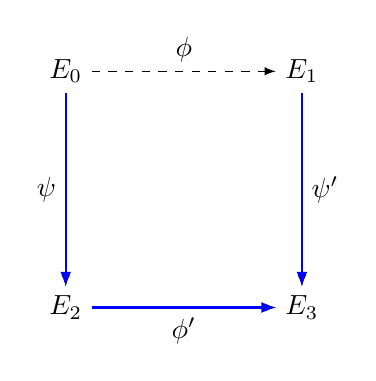
\begin{tikzpicture}
    \node (E0) at (0,0) {$E_0$};
    \node (E1) at (3,0) {$E_1$};
    \node (E2) at (0,-3) {$E_2$};
    \node (E3) at (3,-3) {$E_3$};
    
    \draw[-latex,dashed]
    (E0) edge node[above] {$\phi$} (E1) edge node[left] {$\psi$} (E2)
    (E2) edge node[below] {$\phi'$} (E3)
    (E1) edge node[right] {$\psi'$} (E3);

    \begin{scope}[-latex,thick,blue]
      \uncover<2>{\draw (E0) edge (E2);}
      \uncover<3>{\draw (E1) edge (E3);}
      \uncover<4>{\draw (E2) edge (E3);}
    \end{scope}
  \end{tikzpicture}
\end{frame}

%%

\begin{frame}{Special soundness {\small(as claimed in DFJP11)}}
  \large
  \centering
  \begin{tikzpicture}
    \node (E0) at (0,0) {$E_0$};
    \node (E1) at (3,0) {$E_1$};
    \node (E2) at (0,-3) {$E_2$};
    \node (E3) at (3,-3) {$E_3$};

    \draw[-latex,dashed] (E0) edge (E1);
    \uncover<2->{
      \draw[-latex,blue,thick] (E0) edge (E2) (E2) edge (E3);
    }
    
    \newcount\shift
    \animatevalue<3-6>{\shift}{1}{4}
    \uncover<3-6>{
      \draw[gray,-latex] ($ (E2)!\shift/5!(E0) $) to ($ (E3)!\shift/5!(E1) $);
    }
    \uncover<7->{
      \draw[-latex,blue,thick] (E0) edge (E1);
    }
  \end{tikzpicture}  
\end{frame}

%%

\begin{frame}{Epic fail!}
  \large
  \centering
  \begin{tikzpicture}
    \node (E0) at (0,0) {$E_0$};
    \node (E1) at (7,0) {$E_1$};
    \node (E2) at (2,-3) {$E_2$};
    \node (E3) at (5,-3) {$E_3$};

    \draw[-latex,blue,thick] (E0) edge (E2) (E2) edge (E3) (E1) edge (E3);

    \uncover<2->{
      \draw[-latex,dashed] (E0) edge node[above] {??} (E1);
    }
  \end{tikzpicture}  
\end{frame}

%%

\begin{frame}{Our (not) elegant fix!}
  \large
  \centering
  \begin{tikzpicture}
    \node (E0) at (0,0) {$E_0$};
    \node (E1) at (7,0) {$E_1$};

    \node[draw,gray] (E2) at (0,-3) {$E_2[B] = \langle P_2,Q_2\rangle$};
    \node[draw,gray] (E3) at (7,-3) {$E_3[B] = \langle P_3,Q_3\rangle$};
    
    \uncover<2->{
      \node[draw,gray] (ab) at (3.5,-1.5) {$a,b$};
    }

    \uncover<3,6->{
      \node[draw,dashed,blue] at (E2) {$E_2[B] = \langle P_2,Q_2\rangle$};
      \node[draw,dashed,blue] at (E3) {$E_3[B] = \langle P_3,Q_3\rangle$};
      \draw[-latex,thick,blue] (E2) edge node[below] {$\phi'$} (E3);
    }

    \uncover<4,10->{
      \node[draw,dashed,blue] at (E2) {$E_2[B] = \langle P_2,Q_2\rangle$};
      \node[draw,dashed,blue] at (ab) {$a,b$};
      \draw[-latex,thick,blue] (E2) edge node[left] {$\widehat\psi$} (E0);
    }
    
    \uncover<5->{
      \node[draw,dashed,blue] at (E3) {$E_3[B] = \langle P_3,Q_3\rangle$};
      \node[draw,dashed,blue] at (ab) {$a,b$};
      \draw[-latex,thick,blue] (E3) edge node[right] {$\widehat\psi'$} (E1);
    }

    \uncover<3->{
      \node[red] at (1,-5) {$P_3 = \phi'(P_2),\qquad Q_3 = \phi'(Q_2)$};
    }
    \uncover<4->{
      \node[red] at (1,-5.7) {$\ker\widehat\psi = aP_2+bQ_2$};
    }
    \uncover<5->{
      \node[red] at (1,-6.4) {$\ker\widehat\psi' = aP_3+bQ_3$};
    }

    \newcount\shift
    \animatevalue<6-9>{\shift}{1}{4}
    \uncover<6-9>{
      \draw[gray,-latex] ($ (E3)!\shift/5!(E2) $) to ($ (E1)!\shift/5!(E0) $);
    }
    
    \uncover<10->{
      \node at (5,-5.7) {\LARGE$\Bigg\}\Rightarrow$};
      \node at (7.5,-5.3) {$\ker\widehat\psi' = \phi'(\ker\widehat\psi)$};
    }

    \animatevalue<11-14>{\shift}{1}{4}
    \uncover<11-14>{
      \draw[gray,-latex] ($ (E2)!\shift/5!(E0) $) to ($ (E3)!\shift/5!(E1) $);
    }

    \uncover<15->{
      \draw[-latex,thick] (E0) edge node[above] {$\phi$} (E1);
      \node at (7.5,-6.1) {$\ker\phi = \widehat\psi(\ker\phi')$};
    }
  \end{tikzpicture}  
\end{frame}

%%

\begin{frame}{Zero-knowledge}
  \large
  \centering
  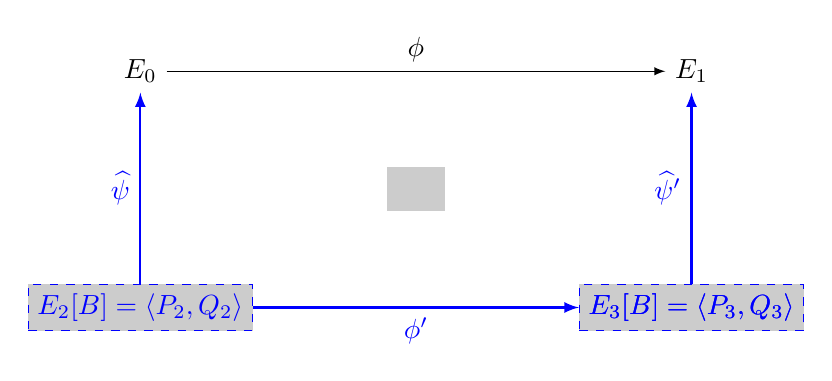
\begin{tikzpicture}
    \node (E0) at (0,0) {$E_0$};
    \node (E1) at (7,0) {$E_1$};
    \node[draw,gray] (E2) at (0,-3) {$E_2[B] = \langle P_2,Q_2\rangle$};
    \node[draw,gray] (E3) at (7,-3) {$E_3[B] = \langle P_3,Q_3\rangle$};
    \node[draw,gray] (ab) at (3.5,-1.5) {$a,b$};

    \draw[-latex] (E0) edge node[above] {$\phi$} (E1);

    \uncover<1>{
      \node[draw,dashed,blue] at (E2) {$E_2[B] = \langle P_2,Q_2\rangle$};
      \node[draw,dashed,blue] at (ab) {$a,b$};
      \fill[black!20!white] (E3.north east) rectangle (E3.south west);
      \draw[-latex,thick,blue] (E2) edge node[left] {$\widehat\psi$} (E0);
    }

    \uncover<2>{
      \node[draw,dashed,blue] at (E3) at (7,-3) {$E_3[B] = \langle P_3,Q_3\rangle$};
      \node[draw,dashed,blue] at (ab) {$a,b$};
      \fill[black!20!white] (E2.north east) rectangle (E2.south west);
      \draw[-latex,thick,blue] (E3) edge node[left] {$\widehat\psi'$} (E1);
    }

    \uncover<3>{
      \node[draw,dashed,blue] at (E2) {$E_2[B] = \langle P_2,Q_2\rangle$};
      \node[draw,dashed,blue] at (E3) at (7,-3) {$E_3[B] = \langle P_3,Q_3\rangle$};
      \fill[black!20!white] (ab.north east) rectangle (ab.south west);
      \draw[-latex,thick,blue] (E2) edge node[below] {$\phi'$} (E3);
    }
  \end{tikzpicture}

  \vfill
  
  \uncover<3->{
    \emph{Assumption:} Decisional Supersingular Product (DSSP)
  }
\end{frame}

%%

\begin{frame}{Statistical ZK (BCCDFLMPPW '22)}
  \large
  \centering
  \begin{tikzpicture}
    \newcount\shift
    \animatevalue<1-4>{\shift}{0}{3}
    
    \node (E0) at (0,0) {$E_0$};
    \node (E1) at (3,0) {$E_1$};
    \node (E2) at (0,-3-\the\shift) {$E_2$};
    \node (E3) at (3,-3-\the\shift) {$E_3$};

    \draw[-latex] (E0) edge (E1) (E2) edge (E3);
    \draw[-latex,dashed] (E0) edge (E2);

    \draw[gray] (6,1) -- ++(0,-8);
    \node at (6,-3) {\LARGE\alt<4->{$\approx$}{??}};

    \node (F0) at (9,0) {$E_0$};
    \node (F1) at (12,0) {$E_1$};
    \node (F2) at (9,-3-\the\shift) {$E_2$};
    \node (F3) at (12,-4.5-\the\shift/2) {$E_3$};

    \draw[-latex] (F0) edge (F1) (F2) edge (F3);
    \draw[-latex,dashed] (F0) edge (F2);
    
  \end{tikzpicture}
\end{frame}

%%

\begin{frame}{Summary}
  \large
  
  This work:
  \begin{itemize}
  \item A \emph{knowledge sound}, \emph{computational ZK} protocol to
    prove knowledge of an isogeny walk\dots It was about time!
  \item A variant to prove \emph{knowledge of an SIDH key}\dots
    Because, why not?
  \end{itemize}

  \bigskip

  Recent development:
  \begin{itemize}
  \item A \emph{statistically ZK} protocol for the same\dots but
    knowledge soundness not as good.
  \end{itemize}

  \bigskip

  Open problems:
  \begin{itemize}
  \item Statistical ZK + strong Knowledge soundness.
  \item Efficiency.
  \item An even remotely efficient protocol for the CSIDH setting:\\
    (SeaSign sucks and CSI-FiSh doesn't scale).
  \end{itemize}
\end{frame}

\end{document}


% LocalWords:  Isogeny abelian isogenies hyperelliptic supersingular Frobenius
% LocalWords:  isogenous
